
\documentclass{article}%

\usepackage{amsmath}%
\usepackage{amsfonts}%
\usepackage{amssymb}%
\usepackage{graphicx}
\usepackage[english,greek]{babel}
\usepackage[utf8x]{inputenc}
\usepackage{listings}
\usepackage{lipsum}
\begin{document}


\selectlanguage{greek}

\title{Δίκτυα Επικοινωνιών\\5η εργαστηριακή άσκηση\\ 
Επίδοση πρωτοκόλλου \textlatin{Selective Repeat}}
\author{Γεώργιος Δασούλας\\Α.Μ: 03112010 \\ 6ο Εξάμηνο 2014-2015  }
\date{\today}
\maketitle

Στη συγκεκριμένη άσκηση θα μελετηθεί η χρησιμότητα και η επίδοση του πρωτοκόλλου \textlatin{Selective Repeat}.Το πρωτόκολλο αυτό
μπορεί να χρησιμοποιηθεί, εκτός από το στρώμα ζεύξης δεδομένων, και στο στρώμα μεταφοράς, ώστε να
παρέχεται υπηρεσία με εγγυημένη παράδοση δεδομένων πάνω από αναξιόπιστο δίκτυο. Παρακάτω, βρίσκεται η τοπολογία που χρησιμοποιείται για τη συγκεκριμένη άσκηση.
\begin{figure}[htbp]
	\centering
		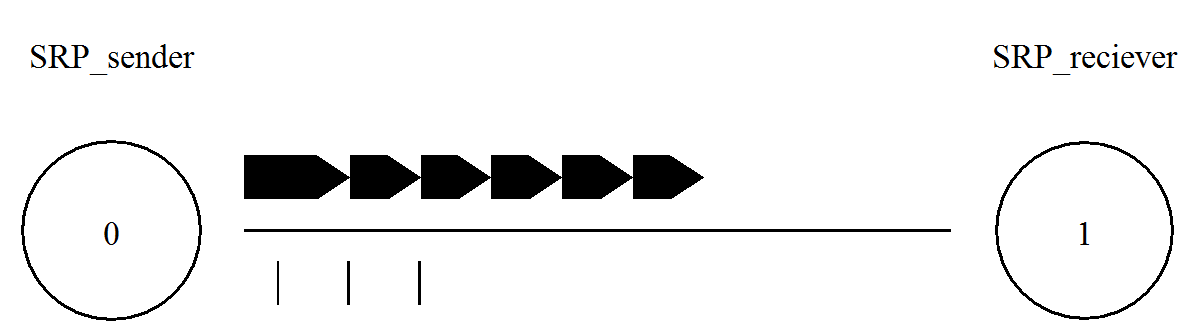
\includegraphics[width=0.50\textwidth]{1.png}
	\label{fig:1}
\end{figure}

\textbf{\underline{ Απαντήσεις ερωτήσεων}}\\
\begin{itemize}
	\item  (α) Πώς πρέπει να τροποποιηθεί ο κώδικας της προσομοίωσης ώστε η ζεύξη μεταξύ των δύο κόμβων
της διάταξης να απεικονίζεται σε οριζόντια θέση, όπως φαίνεται στο Σχήμα 1$?$ \\
\textbf{Απάντηση}: Αρκεί να τοποθετήσουμε μετά τη δήλωση της αμφίδρομης ζεύξης την παρακάτω εντολή:
\selectlanguage{english} \verb|$ns duplex-link-op $n(0) $n(1) orient right| .
\selectlanguage{greek} Έτσι, ορίζουμε τον προσανατολισμό της ζεύξης, ρυθμίζοντάς την οριζόντια.\\
\newpage
\item	Να επαληθεύσετε κατά πόσον ισχύει ή όχι η εξίσωση σε περίπτωση απουσίας σφαλμάτων: $\displaystyle{\eta=min\{\frac{W \times TRANSP}{S},1\}}$.\\
\textbf{Απάντηση}:Έχουμε : \\$W = 10$\\
$TRANSP=\frac{packet\_length}{transfer\_rate}=\frac{1500*8bits}{2Mbits/sec}=\frac{7680bits}{2Mbits/sec}=0.00384$ $sec$\\
$PROP= 40$ $ms$\\
$TRANSA=\frac{40*8}{2Mbits/sec}=0.00016$ $sec$ ( το μήκος της επιβεβαίωσης =40 $bytes$ το εντοπίσαμε στο $.tr$ αρχείο )\\
$S=2*TRANSP + PROP + 2*TRANSA = 0.084$ $sec$\\
Άρα, η θεωρητική τιμή του $\eta=min\{0.47619,1\}=0.47619$ $sec$. 
Επίσης, από το αρχείο $awk$ βρίσκουμε τον πραγματικό ρυθμό μετάδοσης των δεδομένων:
\begin{figure}[htbp]
	\centering
		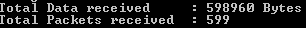
\includegraphics[width=0.30\textwidth]{2.png}
	\label{fig:2}
\end{figure}\\
Έχουμε ,λοιπόν, για την πειραματική τιμή $\eta = \frac{598960*8bits}{5.33144-0.25}*\frac{1}{2Mbits\sec}=0.4715$ $sec$.
Άρα, η θεωρητική και η πειραματική τιμή της επίδοσης του πρωτοκόλλου συγκλίνουν.\\

\item	(γ) Ποιος είναι ο αριθμός των πακέτων που παρελήφθησαν; Πόσα δεδομένα παρελήφθησαν από τον
παραλήπτη κατά τη διάρκεια της προσομοίωσης $?$
\textbf{Απάντηση}:	Όπως φαίνεται και στην προηγούμενη εικόνα από τα αποτέλεσματα του $awk$ προέκυψε πως : παρελήφθησαν 599 πακέτα και συνολικά 598960 $Bytes$. Από αυτά τα νούμερα φαίνεται , επίσης, πως ενώ όλα τα πακέτα μεταφέρουν 1000 $bytes$ , το πρώτο μεταφέρει 960 $bytes$.
\\
\item	(δ) Τροποποιήστε κατάλληλα το πρόγραμμα $awk$, ώστε να προσδιορίζει τη συνολική διάρκεια
μετάδοσης των δεδομένων (η οποία περιλαμβάνει και την ολοκλήρωση μετάδοσης όλων των
επιβεβαιώσεων). Υπολογίστε το ρυθμό μετάδοσης δεδομένων και τη χρησιμοποίηση του καναλιού. 
\textbf{Απάντηση}:\\ Αρκεί να κρατήσουμε σε δύο μεταβλητές την αρχική και την τελική χρονική στιγμή, η οποίο στο $tr$ αρχείο απεικονίζεται στη δεύτερη λέξη. Οπότε, το αρχείο μπορεί να τροποποιηθεί ως εξής:
\selectlanguage{english}
\begin{verbatim}
BEGIN {
	data=0;
	packets=0;
	finished=0.0;
}
/^r/&&/tcp/ {
	data+=$6;
	packets++;
}
/^r/&&/ack/ {
	finished = $2; }
END{
	printf("Total Data received\t: %d Bytes\n", data);
	printf("Total Packets received\t: %d\n", packets);
	printf("Last ack packet received\t: %f\n",finished);
}
\end{verbatim}
\selectlanguage{greek} Προέκυψε ότι η συνολική διάρκεια αποστολής πακέτων είναι : 5.08144 $seconds$.  Άρα, ο ρυθμός μετάδοσης των δεδομένων είναι :$\frac{598960*8}{5.08144}=942976.794$ $bits/sec$. Επίσης, η χρησιμοποίηση του καναλιού είναι $\frac{942976.794 bits/sec}{2Mbits/sec}=47.14\%$.
\item	(ε) Με βάση την εξίσωση που παρατίθεται νωρίτερα, υπολογίστε τη θεωρητική τιμή της
χρησιμοποίησης του καναλιού, θεωρώντας ότι το μέγεθος των πακέτων αυξάνεται κατά 40 $byte$
λόγω επικεφαλίδων $TCP$ και $IP$, και ότι οι επαληθεύσεις ($ACK$) έχουν μέγεθος 40 $byte$. Ισχύει η
εξίσωση; Αν όχι, πού οφείλεται η απόκλιση $?$\\
\textbf{Απάντηση}: To $W=10$ παραμένει ίδιο . Επίσης, $TRANSP=8000/2Mbits/sec=4$ $ms$,  $TRANSA=320/2000000=0.16$ $ms$.Άρα, προκύπτει $\eta= min\{10*0.04/0.08416,1\}=0.47528$. Βλέπουμε πως η θεωρητική τιμή είναι λίγο μεγαλύτερη από την πειραματική.Η απόκλιση αυτή πιθανώς να οφείλεται στην καθυστέρηση μεταξύ λήψης πακέτου και της αποστολής της επιβεβαίωσης.\\
\item	(στ) Διατηρώντας σταθερό το μέγεθος του παραθύρου, αλλάξτε το μήκος των πακέτων, ώστε η
θεωρητική απόδοση του πρωτοκόλλου να λάβει τη μέγιστη τιμή της. Για ποιο μήκος πακέτων
συμβαίνει αυτό; Υπολογίστε πειραματικά την απόδοση του πρωτοκόλλου (χρησιμοποίηση του
καναλιού) για το μήκος πακέτου που προσδιορίσατε εδώ. Υπάρχει απόκλιση μεταξύ πειραματικής
και θεωρητικής τιμής $?$\\
\textbf{Απάντηση}: Θεωρώντας ως μέγιστη απόδοση τη μοναδιαία βρίσκουμε μήκος πακέτων ίσο με $packetsize=2231 bytes$. Άρα, από την εφαρμογή του $awk$ αρχείου προέκυψε :ρυθμός μετάδοσης $1968473.14 bits/sec$. Άρα, η απόδοση είναι $\frac{1968473.14}{2000000}=0.981$. Παρατηρούμε κι εδώ απόκλιση , η οποία οφείλεται στο ότι το μεγαλύτερο μήκος πακέτου προκαλεί μεγαλύτερη καθυστέρηση μεταξύ παραλαβή του πακέτου δεδομένων και αποστολή του πακέτου επιβεβαίωσης.\\
\item	(ζ) Διατηρώντας το μήκος πακέτου που υπολογίσατε στο ερώτημα (στ), αυξήστε (AM1
+6) φορές το
ρυθμό μετάδοσης της ζεύξης και ρυθμίστε το μέγεθος του παραθύρου, ώστε και πάλι η απόδοση να
λάβει τη μέγιστη τιμή της. Για ποιο μέγεθος παραθύρου συμβαίνει αυτό; Πόσα περισσότερα $bits$
απαιτούνται για την αναπαράσταση των αριθμών ακολουθίας πακέτων του πρωτοκόλλου $Selective$
$Repeat$ στην περίπτωση αυτή$?$\\
\textbf{Απάντηση}:Αυξάνουμε το ρυθμό μετάδοσης της ζεύξης 6 φορές. Άρα , έχουμε νέο ρυθμό μετάδοσης $12Mbits/sec$. Και πάλι θέλουμε μέγιστη τιή για την απόδοση , δηλαδή τη μοναδιαία. Άρα, έχουμε : $W=\frac{S}{TRANSP}=\frac{TRANSP+2*PROP+TRANSA}{2231*8/12Mbits/sec}= \frac{1.487+2*40+0.026}{1.487}=54.81=55$. Ισχύει $W=\frac{1+max\_seq}{2}\Rightarrow max\_seq=109$, που στο δυαδικό σύστημα χρειάζεται 7 $bits$. Πριν είχαμε $W=10$ , δηλαδή $max\_seq=9$, που αναπαρίσταται με 5 $bits$. Άρα, χρειαζόμαστε 2 παραπάνω $bits$.\\
\item	(η) Εφαρμόστε τώρα το πρωτόκολλο για την παραμετροποίηση του ερωτήματος (ζ), θεωρώντας όμως
ζεύξη με πενταπλάσια καθυστέρηση διάδοσης. Υπολογίστε την απόδοση του πρωτοκόλλου στη νέα
αυτή ζεύξη τόσο θεωρητικά, όσο και πειραματικά. Αιτιολογείστε τυχόν αποκλίσεις που
παρατηρούνται.\\ 
\textbf{Απάντηση}:Αλλάζουμε τις αντίστοιχες εντολές στον κώδικά μας.\selectlanguage{english} \verb|$tcp0 set window_ 127|\\

\verb|$tcp0 set windowInit_ 127| \selectlanguage{greek} και ρυθμίζουμε και το ρυθμό μετάδοσης της αμφίδρομης ζεύξης στα $12Mbits/sec$. Προκύπτουν τα αποτελέσματα : 
\begin{figure}[htbp]
	\centering
		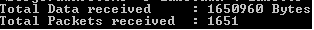
\includegraphics[width=0.40\textwidth]{3.png}
	\label{fig:3}
\end{figure}
Άρα, η πειραματική τιμή είναι $\frac{1650960*8}{5.542987-0.25}=2495316.92 bits/sec$. Άρα, η απόδοση είναι $\eta= \frac{2495316.92}{12000000}=0.2079$. Για τη θεωρητική τιμή χρησιμοποιούμε τις ίδιες εξισώσεις με πρίν και βρίσκουμε $\eta=0.20852$. Βλέπουμε ότι υπάρχει μικρή απόκλιση , η οποία μπορεί να οφείλεται στη διαφορά των $bits$ που χρειάζονται για την αναπάρασταση. 
\item	(θ) Εφαρμόστε το πρωτόκολλο \textlatin{Go Back N} αντί του \textlatin{Selective Repeat} στην τελευταία παραμετροποίηση
της προσομοίωσης και μετρήστε την απόδοση του πρωτοκόλλου αυτού πειραματικά. Διαφέρουν οι
πειραματικές αποδόσεις των δύο πρωτοκόλλων $?$ Γιατί $?$ \\
\textbf{Απάντηση}: Αλλάζουμε την εντολή ορισμού $tcp$ σε \selectlanguage{english} \verb|set tcp0 [new Agent/TCP/Reno]|,\selectlanguage{greek} βρίσκουμε πως τρέχοντας το $awk$ αρχείο βρίσκουμε τα ίδια αποτελέσματα, καθώς δεν υπάρχουν σφάλματα, γιατί αν υπήρχαν τότε το πρωτόκολλο $Selective$ $Repeat$ θα είχε καλύτερη απόδοση.
\begin{figure}[htbp]
	\centering
		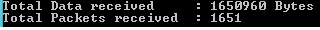
\includegraphics[width=0.40\textwidth]{4.png}
	\label{fig:4}
\end{figure}
 \\

\end{itemize}

\end{document}
